\section{Beispiele}

Das Ziel dieses Abschnittes ist es, dem Benutzer die Verwendung von
Intervall-Events näherzubringen. Dazu wird gezeigt, an welchen Stellen sich
Intervall-Events sinnvoll einsetzen lassen. Bis auf das letzte Beispiel
existieren für alle Beispiele zwei Implementierungen. Eine Implementierung die
Intervall-Events verwendet und eine Implementierung die keine Events
verwendet.

\subsection{Implementierung eines Zustandsautomaten}
Zwei Beispiele zeigen die Verwendung von Intervall-Events bei der
Implementierung von Zustandsautomaten. Zustandsautomaten k"onnen hervoragend
durch die Verwendung von IntervallEvents implementiert werden, da
Zustandsautomaten immer vom Zustand abh"anige Reaktionen auf Events zeigen.

Zur Implementierung kann jeder Zustand des Automaten als ein Intervall
abgebildet werden. Alle in einen Zustand eingehende Transitionen werden dabei
als Start-Events des Intervalls verwendet und alle vom Zustand ausgehende
Transitionen werden als End-Event des Intervalls verwendet. Alternativ könnte
man auch die \after{}-Events des vorherigen Zustandsintervalls als Startevent
des nächsten Zustandes verwenden.

Durch diese Vorgehensweise ergibt sich eine bessere Wartbarkeit des
Quellcodes, da das Programmverhalten nicht mehr imperativ durch If-Statements
oder das Statemachine-Pattern beschrieben wird. Viel mehr wird das
Programmverhalten deklarativ durch Intevall-Events spezifiziert.

Im Rahme dieser Arbeit wurden zwei Zustandsautomaten implementiert. Der erste
Zustandsautomat besteht aus zwei Zuständen und soll dem Benutzer die
Vorgehensweise zur Implementierung eines Zustandsautomaten an einem stark
vereinfachten Beispiel zeigen. Der resultierende Zustandsautomat ist in Abb.
\ref{filetransfer_behaviour} zu sehen.

%\usepackage{graphics} is needed for \includegraphics
\begin{figure}[htp]
\begin{center}
  \includegraphics[width=0.15\textwidth]{graphics/tcp_stm.dot.eps}
  \caption{Verhalten einer Filetransfer-Verbindung}
  \label{filetransfer_behaviour}
\end{center}
\end{figure}


Im SimpleWebshop-Beispiel wird eine weitere Herangehensweise an die
Implementierung eines Zustandsautomaten mit Intervall-Events gezeigt. Häufig
lässt sich die Anzahl der benötigten Zustände und Transitionen durch die
Verwendung von paralellen oder hierarchischen Zustandsautomaten reduzieren.
Damit wird das Modell leichter verständlich aber die Implementierung des Modells
erschwert. 
Besonders die Implementierung von paralellen Zustandsautomaten ist zumeist sehr
unpraktisch. Der Zugriff auf den aktuellen Zustand der paralellen
Zustandsautomaten und das Verteilen von Events bereitet nämlich meist
Probleme. Daher werden oft zur Implementierung die Produktautomaten gebildet um
die paralellen Zustände aus dem Modell zu entfernen.

Dies ist bei der Verwendung von Intervall-Events zur Impelmentierung eines
Zustandsautomaten allerdings nicht zwingend notwendig. Die direkte
Implementierung eines paralellen Zustandsautomaten ist ohne Probleme möglich.
Die Verteilung der Events zum Ändern der Zustände und der Zugriff auf
benachbarte Zustandsautomaten ist einfach. 

Die Implementierung eines solchen Zustandsautomaten wie in Abb.
\ref{webshop_behaviour} dargestellt findet sich im Beispiel
interval\_simplewebhop.

%\usepackage{graphics} is needed for \includegraphics
\begin{figure}[htp]
\begin{center}
  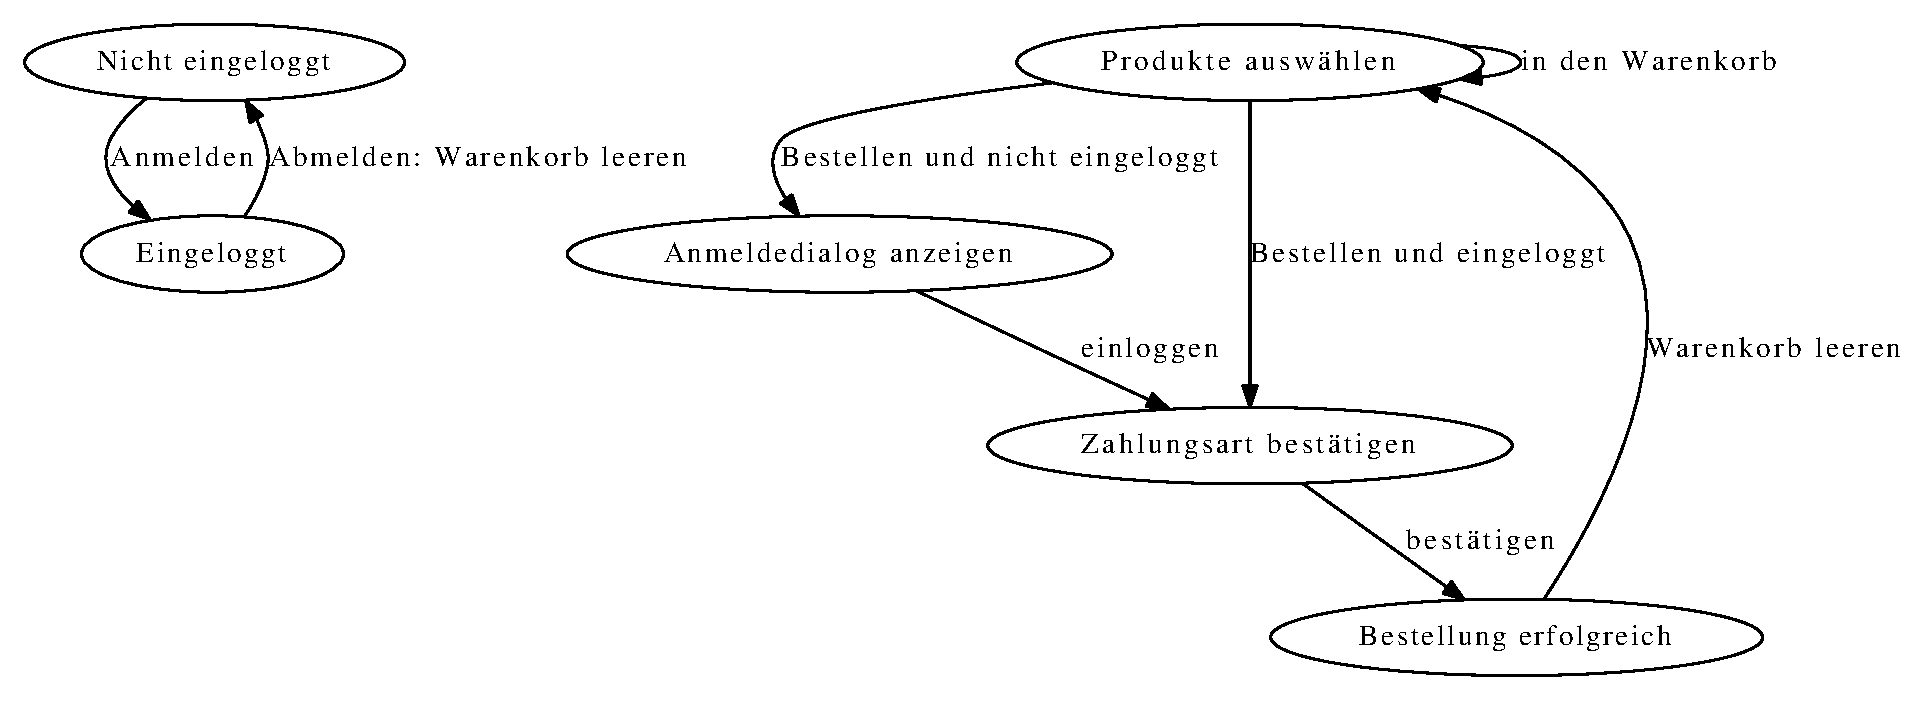
\includegraphics[width=0.6\textwidth]{graphics/webshop.dot.eps}
  \caption{Bestellvorgang in einem Web-Shop}
  \label{webshop_behaviour}
\end{center}
\end{figure}

\subsection{Implementierung einer FileTransfer-Komponente}
In viele Fällen wird ein Softwareentwickler keinen Zustandsautomaten
spezifizieren bevor die Software-Entwicklung beginnt. Viele zu lösende Probleme
lassen sich nämlich durch zwei oder drei Zustände beschreiben, sodass der
Entwickler nicht erst auf die Idee kommt, eine Zustandsmaschine zu
implementieren. Daher stellt sich die Frage, ob Intervall-Events auch in der
Praxis relevant sich um dem Entwickler beim Lösen von alltäglichen Problemen zu
helfen. Das nächste Beispiel zeigt daher die praktische Verwendung von
Intervall-Events:

Mit File-Sharing-Programmen können Benutzer über ein Computernetzwerk
Dateien austauschen. Wenn ein Benutzer eine Dateiübertragung anfordert, dann
fordert das File-Sharing-Programm von unterschiedlichen Hosts Teile der Datei
an. Die Hosts anworten dann mit den angeforderten Dateiteilen. Daher existiert
in den meisten File-Sharing-Programmen eine Komponente zum Steuern der
Dateiübertragungen. Diese Komponente verwaltet die bereits empfangenen
Dateiteile und kümmert sich darum, noch fehlende Tokens nachzufordern.

Bei der Implementierung einer solchen Komponente bietet sich die Verwendung von
Intervall-Events an. Das Verhalten der FileTransfer-Komponente kann fast
vollständig deklarativ erfolgen. 

\subsection{Implementierung von Ping-Pong}
Als größeres Beispiel wurde im Rahmen des Praktikums das Spiel
Ping-Pong implementiert. In diesem Spiel gibt es ein abgegrenztes Spielfeld mit
Wänden. Im Spielfeld befindet sich ein Ball der sich bewegt. Am Spiel teil
nehmen zwei Spieler die jeweils einen eindimensional beweglichen Schläger haben.
Der Schläger befindet sich vor dem Tor des Spielers. Ziel des Spiels ist es, den
Ball nicht in das eigene Tor zu lassen. Als kleine Erweiterung erscheinen auf
der Spielfläche Geschenke die das Spielverhalten abändern. Die Spielfläche des
Spiels ist in Abb. \ref{ping_pong} zu sehen.

\begin{figure}[htp]
\begin{center}
  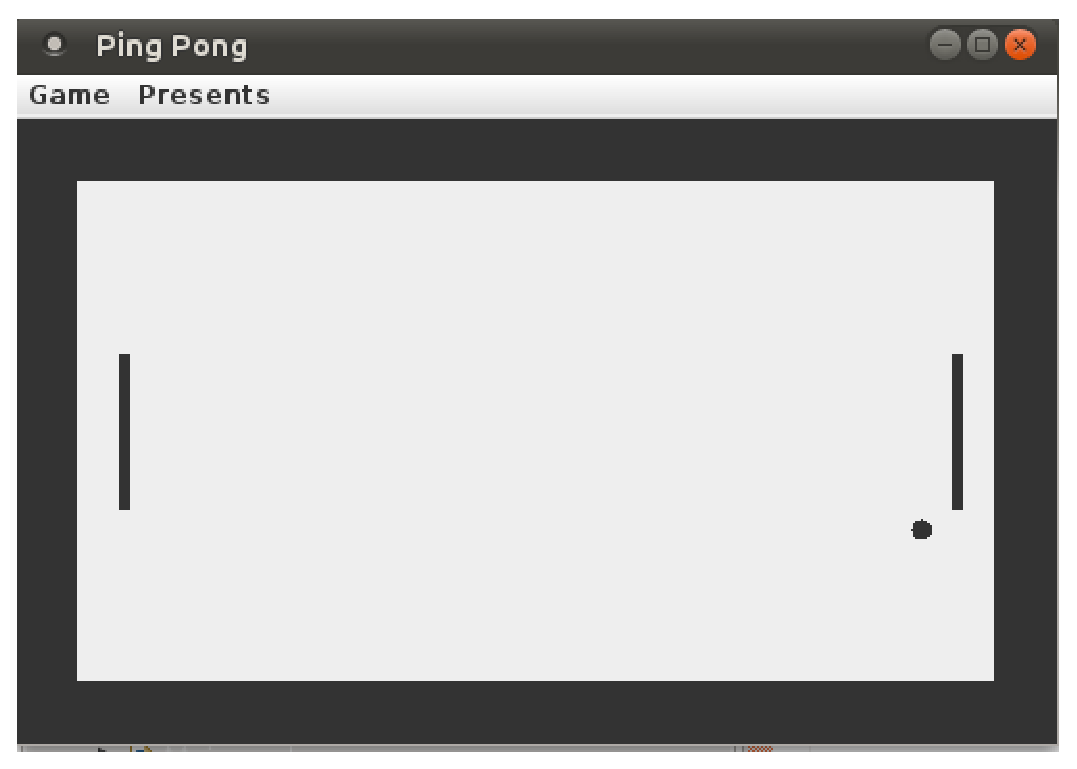
\includegraphics[width=0.6\textwidth]{graphics/pingpong.eps}
  \caption{Ping-Pong}
  \label{ping_pong}
\end{center}
\end{figure}

Das Spielmodell beinhaltet die Wände, den Ball, die Schläger, die Tore und
eventuell Geschenke. Jedes Objekt auf dem Spielfeld hat eine Position und eine
Geschwindigkeit. Allerdings wurde bei der Implementierung des Spiels von der
Klassischen Herangehensweise abgewichen. Klassischerweise besteht ein Spiel aus
einer Spielschleife in der die folgenden Aktionen immer wieder ausgeführt
werden:
\begin{itemize}
  \item Abfragen der Benutzereingaben
  \item Berechnung der Änderungen im Spiel-Modell. Also die Positionsänderung
  des Balls und der Schläger.
  \item Rendern des Spielmodells zu einer Grafik
  \item Warten bis die nächste Iteration notwendig wird. Ohne diese Wartezeit
  hätte man möglicherweise eine zu hohe Frame-Rate.
\end{itemize}

Diese Ansatz ist allerdings nicht Event-Orientiert und wurde daher im Beispiel
nicht verwendet. Stattdesen wird im Beispiel ein Timer verwendet, der alle 50ms
eine Positionsänderung der Objekte und und das Neuzeichnen der Spielfläche auslöst.
Solange ein Spieler eine Bewegen-Taste drückt ist ein Intervall-Event aktiv das
die Geschwindigkeit des Schlägers ändert\footnote{Dies ist übrigens ein
eleganter Workaround für einen Bug in der Java AWT. Mehr Informationen zum
diesem Fehler finden sich unter
bugs.sun.com/view\_bug.do?bug \_id=4153069}.

Weiterhin werden Intervall-Events eingesetzt, um das Zeitmodell des Spiels
abzubilden. Geschenke beispielsweise sollen nur für eine definierte Zeit
vorhanden sein. Diese Funktion wurde durch ein Intervall-Event realisiert, das
vom Beginn der Sichtbarkeit für eine gewisse Zeit aktiv ist. 

\subsection{Zusammenfassung}
Fasst man die Beispiele zu einem Fazit zusammen, so lässt sich sagen, dass durch
die Verwendung von Intervall-Events ein deklaratives Implementieren von
zustandsbasierten Problemen möglich ist. Dies verbessert die Lesbarkeit und die
Wartbarkeit des Quellcodes. Allerdings gibt müssen zwei Schwierigkeiten bei der
Verwendung von Intervall-Events bedacht werden: Zum einen ist Vorsicht bei der
Verwendung von rekursiven Definitionen geboten. Eine Verwendung dieser
Konstrukte erfordert das Markieren des Start-Intervalls mit \textit{lazy} und
die Definition eines Startevents um eine korrekte Initialisierung der rekursiven
Definition vorzunehmen.

Zum anderen ist es wichtig, ein exaktes Event-Modell für eingehende und
ausgehende Events zu erstellen. Es ist wichtig, zwischen Events die Transitionen
auslösen können und Events die Aktionen zur Folge haben zu trennen. Ist diese
Trennung nicht exakt genug, dann könnten eventuell Aktionen ausgeführt werden,
die im akutellen Intervall nicht zulässig sind. 

Beachtet man diese Entwurfskriteren, so ist es durch Intervall-Events möglich,
auf einem hohe Abstraktionsnivea Software zu entwicklen. 
